\documentclass[pdf,9pt,xcolor=dvipsnames,hide notes]{beamer}
\setbeamerfont{page number in head/foot}{size=\large}
\setbeamercolor{footline}{fg=blue}
\setbeamertemplate{footline}[frame number]
\usetheme{CambridgeUS}
\usecolortheme{crane} % or try albatross, beaver, crane, ...
\usepackage{verbatim}
\usefonttheme{serif}     % Font theme: serif
\usepackage{ccfonts}     % Font family: Concrete Math
\usepackage[T1]{fontenc}
\usepackage{lmodern}
\usepackage{caption}
\usepackage[caption=false]{subfig}
\usepackage{tabularx}
\usepackage{booktabs}
\usepackage{pdfpages}
\usepackage{graphicx}  
\usepackage{pgfplots}
\DeclareCaptionLabelSeparator{horse}{:\quad} % change according to your needs
\captionsetup{
	labelsep = horse,
	figureposition = bottom % proper spacing between figure and caption
}
\usepackage{graphicx,amsfonts,booktabs,hyperref,subfig,amssymb,amsmath,amsthm,tabularx,multirow,enumerate}
%\usepackage{parskip}
%\setlength{\parindent}{10pt}
\usepackage{ragged2e,tikz,color,colortbl}
\usepackage[first=0,last=9]{lcg}

\DeclareMathOperator{\Ima}{Im}

% Real Number
\newcommand{\R}{\mathbb R}
% natural numbers
\newcommand{\Nat}{\mathbb N}
% complex numbers
\newcommand{\C}{\mathbb C}
\newcommand{\E}{\mathbb{E}}
\newcommand{\Var}{\mathrm{Var}}
\newcommand{\Cov}{\mathrm{Cov}}
\newcommand{\Corr}{\mathrm{Corr}}
\newcommand{\Expect}{{\rm I\kern-.3em E}}
\newcommand{\backupbegin}{
	\newcounter{finalframe}
	\setcounter{finalframe}{\value{framenumber}}
}
\newcommand{\backupend}{
	\setcounter{framenumber}{\value{finalframe}}
}

\setbeamertemplate{theorems}[numbered]

\setbeamertemplate{caption}[numbered]
\setbeamercolor{postit}{use=structure,fg=black,bg=structure!13!white}
\newcommand{\otoprule}{\midrule[\heavyrulewidth]}
\makeatletter
\newenvironment{withoutheadline}{
	\setbeamertemplate{headline}[default]
	\def\beamer@entrycode{\vspace*{-\headheight}}
}{}
\newcommand{\srcsize}{\@setfontsize{\srcsize}{3.3pt}{3.3pt}}
\makeatother
\title[dasilvafbs@gmail.com]{Pairs Trading: Optimizing via Mixed Copula versus Distance Method for S\&P 500 Assets }
%\subtitle{}
%\author[Department of Statistics (UFRGS)]{\textbf{Fernando A. B. Sabino da Silva}\inst{1}}
%\institute[]{\inst{1} Department of Statistics (UFRGS)}
\author[Department of Statistics (UFRGS)]{\textbf{Fernando A. B. Sabino da Silva}\inst{1}, Flavio A. Ziegelmann\inst{1,2}, Joao F. Caldeira\inst{2}}
\institute[]{\inst{1} Department of Statistics, \inst{2} Graduate Program in Economics, Federal University of Rio Grande do Sul}
%\date{\today} % (optional)
\date{} % (optional)

\hypersetup{
    pdftitle={TITLE},
    pdfauthor={AUTHOR},
    pdfsubject={SUBJECT},
    pdfkeywords={KEYWORD} {KEYWORD} {KEYWORD},
    colorlinks=true,
    linkcolor=blue,
    citecolor=blue,
    filecolor=magenta,
    urlcolor=blue
    }
\usepackage{threeparttable}
\usepackage{pdfpages}  


\begin{document}
	\justifying
	
	\frame{\titlepage}
	
		\section{History}
	
	\begin{frame}[label=frame1]
	\frametitle{History}
	
	\setbeamercovered{transparent}
	
	\begin{itemize}
		\justifying
				
		\item Gerry Bamberger and Nunzio Tartaglia's quantitative group at Morgan Stanley in the early 1980s.
			\begin{itemize}
				\setlength\itemsep{0.5em}
%				\item Morgan Stanley's black box strategy earned the firm a lot of money, and of course, bolster its reputation on Wall Street;
				\pause
				\item David Shaw founded one of the most successfull statistical arbitrage hedge funds to this day (D. E. Shaw \& Co).
				
				\pause
				\item Foundation of statistical arbitrage and consequently, algorithmic trading.
			\end{itemize}
		
		\vspace{0.3cm}
		
		\pause
		\item Pairs Trading is a contrarian strategy designed to generate abnormal profits from the mean-reverting behavior between a pair of stocks. 
		\pause
			\begin{itemize} 
				\item It is well-planned assault on the Efficient Market Hypothesis.
			\end{itemize}
		
			\begin{figure}[htbp]
				\centering
				
\includegraphics[scale=0.5]{algo_trading.png}
			\end{figure}
		
	
	\end{itemize}	
\end{frame}
	
		\section{Two-Dimensional Pairs Trading}	

	\begin{frame}
		\frametitle{Two-Dimensional Pairs Trading}
		
		\begin{figure}[htbp]
			\centering
			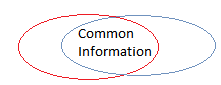
\includegraphics[scale=0.5]{fig1.png}
			\label{fig:fig1}
		\end{figure}
		
		\begin{figure}[htbp]
			\centering
			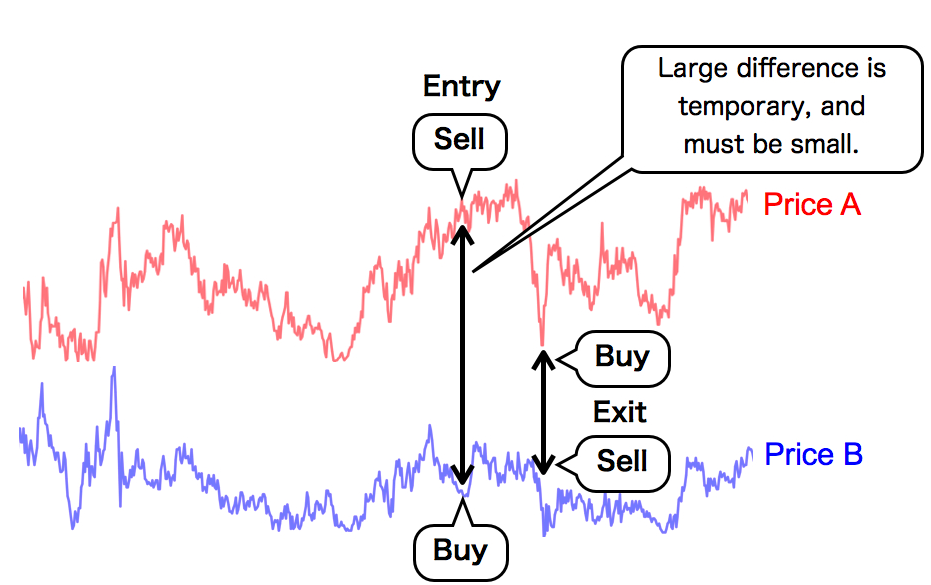
\includegraphics[scale=0.38]{fig2.png}
			\label{fig:fig2}
		\end{figure}
		
	\end{frame}
	
	\section{What is Pairs Trading?}
	
	\begin{frame}[label=frame1]
		\frametitle{What is Pairs Trading?}
		
			
		\begin{itemize}
			\justifying
			
			\setbeamercovered{transparent}
			
			\item Pairs Trading is statistical arbitrage that involves the simultaneous long and short positions of two relatively mispriced stocks which have strong historical co-movements.
			
			\pause
			
			\vspace{0.1cm}
			
			\begin{itemize}
				\setlength\itemsep{1em}
			\item Market-neutral strategy.
			\pause
			\item Self-financing. 
			\pause
			\item Exploit the mean reverting behaviour of co-integrated pairs.
%This means that the investors do not need to invest their own money.
			
		\end{itemize}
			
%			\item The idea is to exploit the mean reverting behaviour of co-integrated pairs. 
%			\begin{itemize}
%				\item If there is a spread between the prices and the further it deviates from its long-term mean value, the greater the probability of a reversal.
%			\end{itemize}
			
			\vspace{0.3cm}
			
			\pause 
			\item However, pairs trading strategy is by no means risk free. 
				\begin{itemize}
					\item Trend rather than mean-reverting.
%					The strategy could perform poorly on stock pairs that pick up a trend rather than mean-reverting.
				\end{itemize}
			
		\end{itemize}
	\end{frame}

	\section{Distance}

\begin{frame}[label=frame1]
\frametitle{Distance Method}

\setbeamercovered{transparent}

\begin{itemize}
	\justifying
			
			\item The most popular strategy is known as distance method (see \textcolor{blue}{Gatev \emph{et al}}., \textcolor{blue}{2006}). 
			
		   \begin{itemize}
		   	\setlength\itemsep{1em}
			
			\item It uses the distance between normalized prices to capture the degree of mispricing stocks. 
			
			\pause
		
			\item According to \textcolor{blue}{Xie \emph{et al}}. \textcolor{blue}{(2014)} the distance method has a multivariate normal nature.
%			 since it assumes a symmetric distribution of the spread between normalized prices of the stocks within a pair and it uses a single distance measure, which can be seen as an
				\begin{itemize} 
			 	\item Alternative measurement of the linear association.
			 	%, to describe the relationship between two stocks.
			 	% asymmetric conditional variance, nonlinear temporal dependence
				\end{itemize}
			\end{itemize}
			
		\end{itemize}	
	\end{frame}


\begin{frame}
%\frametitle{Bivariate Normal Distribution}
	
\begin{exampleblock}{Bivariate Normal Distribution}

\[
f(x,y)=\frac{\exp \left\{ -\frac 1{2(1-\rho ^2)}\left[ \left( \frac{x-\mu _x%
	}{\sigma _x}\right) ^2-2\rho \left( \frac{x-\mu _x}{\sigma _x}\right) \left( 
	\frac{y-\mu _y}{\sigma _y}\right) +\left( \frac{y-\mu _y}{\sigma _y}\right)
	^2\right] \right\} }{2\pi \sigma _x\sigma _y\sqrt{1-\rho ^2}} 
\]

%where $(\mu _x,\mu _y)$ is the mean vector and the variance-covariance
%matrix is
%
%\[
%\left( 
%\begin{array}{cc}
%Var(X) & Cov(X,Y) \\ 
%Cov(X,Y) & Var(Y)
%\end{array}
%\right) =\left( 
%\begin{array}{cc}
%\sigma _x^2 & \rho \sigma _x\sigma _y \\ 
%\rho \sigma _x\sigma _y & \sigma _y^2
%\end{array}
%\right), 
%\]
%
%where $\sigma _x>0, \sigma _y>0$ and $-1<\rho <1.$

\end{exampleblock}

\def\centerx{2}
\def\centery{-1}

	\begin{tikzpicture}[thick,scale=0.8, every node/.style={scale=0.8}]
		\begin{axis}
			\addplot3[surf,domain=-2:6,domain y=-5:3] 
			{exp(-( (x-\centerx)^2 + (y-\centery)^2)/3 )};
			\node[circle,inner sep=1pt,fill=blue,pin=90:$\mu$] 
			at (axis cs:\centerx,\centery,1) {};
			\end{axis}
			
		\hspace{6cm}
			\begin{figure}[!h]
				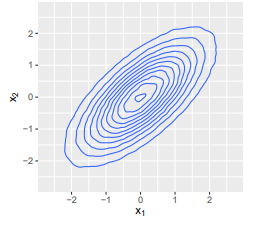
\includegraphics[scale=0.7]{taildep_gaussian.png}
			\end{figure}
			
	\end{tikzpicture}
	
\end{frame}
	
	
	\begin{frame}[label=frame1c]
		\frametitle{Motivation}
		
		\setbeamercovered{transparent}
		
		\begin{itemize}
			\justifying
			
			\item Linear correlation ($\rho$) fully describes the dependence between securities if the series have joint normal distribution. 
			
			\pause
			
			\vspace{0.3cm}
			
			\item  Tail dependence
				\begin{itemize}
					\item Heavy tails.
					\item Possibly Asymmetric.
				\end{itemize}
			
			% is the presence of heavy and possibly asymmetric tails. 
			
%			 However, a main feature of joint distributions characterized by 
	\vspace{0.3cm}
	
	\pause
			
		\item A single distance measure may fail to catch the dynamics of the spread between a pair of securities.
		
	\pause
		\begin{itemize}
			\item Initiate and close the trades at non-optimal positions.
		\end{itemize}

	\pause	
			\vspace{0.3cm}
			
			\item \textcolor{blue}{Lie and Wu} \textcolor{blue}{(2013)} proposed a pairs trading strategy based on 2-dimensional copulas to overcome the limitations of the distance method.
			
			\vspace{0.3cm}
			
		
		\end{itemize}
	\end{frame}

\section{Copula}
	
		\begin{frame}[label=frame1c2]
	\frametitle{Sklar's Theorem (1959)}
	
	
\begin{theorem}
	Let $X_{1},...,X_{d}$ be random variables with distribution functions $F_{1},...,F_{d}$, respectively. Then, there exists an d-copula C such that,
	\begin{equation}
	F\left( x_{1},...,x_{d}\right) =C\left( F_{1}\left( x_{1}\right)
	,...,F_{d}\left( x_{d}\right) \right) ,  \label{1} 
	\end{equation}
\noindent for all $\mathbf{x}=\left( x_{1},...,x_{d}\right) \in
\mathbb{R}^{d}$. If $F_{1},...,F_{d}$ are all continuous, then the function $C$ is unique; otherwise $C$ is determined only on $\Ima F_{1}\times ...\times \Ima F_{d}$. 
\end{theorem}

%\begin{itemize}
%	\item Conversely, if $C$ is an $n$-copula and $F_{1},...,F_{d}$ are distribution functions, then the function $F$ defined above is an $d$-dimensional distribution function with marginals $F_{1},...,F_{d}$.
%\end{itemize}

\end{frame}

\begin{frame}[label=frame2]
\frametitle{Why should we care about copulas?}

\setbeamercovered{transparent}

	\begin{itemize}
		\justifying
		
		\item Assuming that $F\left( \cdot \right) $ and $C\left( \cdot
		\right) $ are differentiable, by $\left( \ref{1}\right)$ we have
		
	\end{itemize}
	
	\begin{eqnarray}
	\frac{\partial ^{d}F\left( x_{1},...,x_{d}\right) }{\partial
		x_{1}...\partial x_{d}} &\equiv &f\left( x_{1},...,x_{d}\right) =\frac{
		\partial ^{d}C\left( F_{1}\left( x_{1}\right) ,...,F_{d}\left( x_{d}\right)
		\right) }{\partial x_{1}...\partial x_{d}} \\
	&=&c\left( u_{1},...,u_{d}\right) \prod_{i=1}^{d}f_{i}\left( x_{i}\right),
	\label{23}
	\end{eqnarray}%
	where $u_{i}$=$F_{i}\left( x_{i}\right) $, $i=1,...,d$.
	
	\vspace{0.3cm}
	\pause
	
	\begin{itemize}
		\item Estimate the multivariate distribution in two parts: (i) finding the marginal distributions; (ii) finding the dependency between the filtered data from (i). 
	\end{itemize}

	
	%From a modelling perspective, Sklar's Theorem allow us to
	
\end{frame}

\begin{frame}[label=frame4b]
	\frametitle{Copula}
	
	\setbeamercovered{transparent}
	
	\begin{itemize}
	\justifying
		
		\item Any multivariate joint distribution can be written in terms of their univariate marginal distribution function and the dependence structure (represented in $C$) between the variables.
		%Sklar's theorem states that
		
		\pause
		\vspace{0.3cm}
		
		\item Copulas accommodate various forms of dependence through suitable choice of the copula ``correlation matrix'' since they conveniently se \linebreak parate marginals from dependence component.
		
		\pause
		\vspace{0.3cm}
		
%		\definecolor{bluegreen}{rgb}{0.0, 0.87, 0.87}
%		\definecolor{amber}{rgb}{1.0, 0.75, 0.0}
%		\definecolor{celadon}{rgb}{0.67, 0.88, 0.69}
%		\definecolor{citrine}{rgb}{0.89, 0.82, 0.04}
		\definecolor{corn}{rgb}{0.98, 0.93, 0.36}
%		\definecolor{darkorange}{rgb}{1.0, 0.55, 0.0}
%		\definecolor{deepsaffron}{rgb}{1.0, 0.6, 0.2}
%		\rowcolor{bluegreen}
%		\rowcolor{amber}
%		\rowcolor{celadon}
%		\rowcolor{citrine}
%		\rowcolor{corn}
%		\rowcolor{darkorange}
%		\rowcolor{deepsaffron}
		
		\begin{table}[ht]
			\centering
			\begin{tabular}{c|ccccccc}
				\hline
				\rowcolor{corn}
				Strategy & Associations & Required Marginal \\
				\rowcolor{corn}
				& Captured & Distributions \\
				\hline
				Distance& Linear & Gaussian \\
				Copula& Linear and Nonlinear & No assumption \\
				\hline
			\end{tabular}
		\end{table}
		
	\end{itemize}
\end{frame}

	\section{Data}	

\begin{frame}[label=frame2b]
	\frametitle{Data}
		\begin{itemize}
		\setlength\itemsep{1em}
		\justifying
		
		\item 	\textbf{Sources} Adjusted closing prices, Fama-French factors
		\item \textbf{Universe} All shares that belongs to the S\&P 500 market index  
		%\begin{itemize}
		%	\setlength\itemsep{1em}
		\item \textbf{Dates} July 2nd, 1990 to December 31st, 2015
		\item \textbf{Totals} 1100 stocks during 6426 days
	
		% \item Eliminate survivorship bias 
		%	\item Bloomberg
		%	\item Fama and French factors 
			%and the returns on the from French's website. 
			%We obtain the adjusted closing prices from
			% Daily data of
		\end{itemize}
			%from our database, only stocks that are listed during the formation period are included in the analysis, \emph{i.e.}, around 500 stocks in each trading period.
			%With the objective of eliminating
		
	%\begin{flushright}
	%\hyperlink{counterexample}{\beamerreturnbutton{Counterexample}}
	%\end{flushright}
	
\end{frame}

	\section{Models}
\subsection{Distance}

\begin{frame}[label=frame2c]
\frametitle{Distance: Methodology}

\setbeamercovered{transparent}

\begin{itemize}
\justifying
\item  The matching partner for each stock is found by looking for the security that minimizes the sum of squared deviations between two normalized price series over a twelve-month period (formation period).

	\begin{itemize}
	\item January to December or from July to June.
	\item Adjust them by dividends, stock splits and other corporate actions.
	\end{itemize}

%Specifically, the pairs are formed using data from January to December or from July to June.

%\vspace{0.3cm}
%
%\item Prices are scaled to \$1 at the beginning of each formation period. formation period is set to $1 (price normalization)
%	\begin{itemize}
%	\item They evolve using the return series.
%	\end{itemize}

\vspace{0.3cm}

\pause
\item Select the top 5, 10, $\ldots$, 35 of those combinations that have the smallest sum of squared spreads, allowing re-selection of a specific pair, during the formation period. 

\pause
	\begin{itemize}
		\item These pairs are then traded in the next six-month period (trading period).
	\end{itemize}

\vspace{0.3cm}

\pause 

\item In \textcolor{blue}{Gatev \emph{et al}}. \textcolor{blue}{(2006)}, the long-short position is opened when pair prices have diverged by 2$\sigma$ and the position is closed when prices revert back.

%when the spread diverges by 2$\sigma$ or more from the mean, the stocks are assumed to be mispriced in terms of their relative value to each other.
% (which is calculated in the formation period
% and thus we open a short position in the outperforming stock and a long in the underperforming one. 

\end{itemize}

\end{frame}

\begin{frame}[label=frame3]
	\frametitle{Pairs Methodology}
	
	\setbeamercovered{transparent}
	
	\begin{itemize}
		\justifying
		\item To calculate the daily percentage excess returns for a pair, we compute
		\begin{equation}
		\begin{aligned}
		r_{pt}=w_{1t}r_{t}^{L}-w_{2t}r_{t}^{S},
		\end{aligned}
		\label{eq:eq01}
		\end{equation}
		where $L$ and $S$ stands for long and short, respectively. 
		
		\vspace{0.3cm}
		
		%To calculate the daily percentage excess returns for a pair, we compute
		
		\item The weights $w_{1t}$ and $w_{2t}$ are initially assumed to be one. After that, they change according to the changes in the value of the stocks, \emph{i.e.}, $w_{it}=w_{it-1}(1+r_{it-1})$.
		
		\vspace{0.3cm}
		
		\pause
		\item  Committed capital and fully invested capital. 
		% Following \textcolor{blue}{Gatev \emph{et al}}. \textcolor{blue}{(2006)}, We calculate returns using two weighting schemes: the return on
	
	\end{itemize}
	
\end{frame}

\begin{frame}[label=frame2d]
	\frametitle{Distance}
		\section{Methodology}
		
		\setbeamercovered{transparent}

\begin{itemize}
	\justifying
	
	%		\item The price divergence is expected to be temporary, i.e., the prices are expected to converge to its long-term mean value of 0 (mean-reverting behavior). 
	
	\vspace{0.3cm}
	
	\item Trades that do not converge can result in a loss if they are still open at the end of the trading period when they are automatically closed. 
	
	\pause
	
	\begin{itemize}
		\item Fat left tails.
		% This results
	\end{itemize}
	
	\vspace{0.3cm}
	
	\pause
	\item It may be inappropriate to use constant trigger points because the volatility differs at different price levels.
	
\end{itemize}

%Since the conditional variance is empirically higher for large negative returns and smaller for positive returns, it may be inappropriate to use constant trigger points because the volatility differs at different price levels.

\end{frame}

\begin{frame}[label=frame4e]
	\frametitle{Copula: Methodology}
	
	\setbeamercovered{transparent}
	
	\begin{itemize}
			\item By using the fact that the partial derivative of the copula function gives the conditional distribution function, i.e., 
			
			\begin{eqnarray*}
				P\left( U_{1}\leq u_{1}\left\vert U_{2}=u_{2}\right. \right)  &=&\frac{%
					\partial C\left( u_{1},u_{2}\right) }{\partial u_{2}}=P\left( X_{1}\leq
				x_{1}\left\vert X_{2}=x_{2}\right. \right) , \\
				P\left( U_{2}\leq u_{2}\left\vert U_{2}=u_{1}\right. \right)  &=&\frac{%
					\partial C\left( u_{1},u_{2}\right) }{\partial u_{1}}=P\left( X_{2}\leq
				x_{2}\left\vert X_{1}=x_{1}\right. \right), 
			\end{eqnarray*}
		
		\vspace{0.3cm}
			
			 \textcolor{blue}{Xie \emph{et al}}. \textcolor{blue}{(2014)} define a measure to denote the degree of mispricing.
	
\end{itemize}

\pause

\vspace{0.3cm}
		\begin{definition}
		\begin{itemize}
			\item Let $R_{t}^{X}$ and $R_{t}^{Y}$ represent the random variables of the daily returns of stocks $X$ and $Y$ on time $t$, and
			the realizations of those returns on time t are $r_{t}^{X}$ and $r_{t}^{Y}$, we have
		\end{itemize}
		\begin{eqnarray*}
			MI_{X\mid Y}^{t} & = & P(R_{t}^{X}<r_{t}^{X}\mid R_{t}^{Y}=r_{t}^{Y}) \\
			& \text{and}  & \\
			MI_{Y\mid X}^{t} & = & P(R_{t}^{Y}<r_{t}^{Y}\mid R_{t}^{X}=r_{t}^{X}),
		\end{eqnarray*}
		where $MI_{X|Y}$ and $MI_{Y|X}$ are named the mispricing indexes.
	\end{definition}
\end{frame}

\begin{frame}[label=frame4f]
	\frametitle{Copula: Methodology}
	
%		\vspace{0.3cm}
%	
%		\begin{itemize}
%			\item 	Given current realizations $r_{t}^{X}$ and $r_{t}^{Y}$, if $F_{X}$ and $F_{Y} $ are the marginal distribution functions of $R_{t}^{X}$ and $R_{t}^{Y} $ and C is the copula connecting $F_{X}$ and $F_{Y}$ , we define $u_{1}=F_{X}\left( r_{t}^{X}\right) $ and $u_{2}=F_{Y}\left( r_{t}^{Y}\right) $, and have
%		\end{itemize}
	
				
		\begin{equation}
		\begin{aligned}
		MI_{X\mid Y}^{t}& = &\frac{\partial C(u_{1},u_{2})}{\partial u_{2}} & = & P(R_{t}^{X}<r_{t}^{X}\mid R_{t}^{Y}=r_{t}^{Y}) \\
		& \text{and} & \\
		MI_{Y\mid X}^{t}& = &\frac{\partial C(u_{1},u_{2})}{\partial u_{1}}& = & P(R_{t}^{X}<r_{t}^{X}\mid R_{t}^{Y}=r_{t}^{Y}).
		\end{aligned}
		\label{eq:eq31}
		\end{equation}
		
		\vspace{0.3cm}
		
			\begin{itemize}
			\justifying
			\item A conditional value of 0.5 means that
			the two underlying stocks are considered fairly-valued.
			\end{itemize}
\end{frame}

\begin{frame}[label=frame4f2]
	\frametitle{Copula: Methodology}
	
\setbeamercovered{transparent}
	
	\begin{itemize}
		\item The conditional probabilities, $M_{t}^{X\left\vert Y\right. }$ and $%
		M_{t}^{Y\left\vert X\right. }$, only measure the degrees of relative
		mispricing for a single day. 
		\begin{itemize}
			\item To determine an overall degree of relative
			mispricing we follow \textcolor{blue}{Rad \emph{et al}}. \textcolor{blue}{(2016)}.
		\end{itemize} 
		
		\vspace{0.3cm}
		
		\pause
		
		\item Let $m_{1,t}$ and $m_{2,t}$ be the
		overall mispricing indexes of stocks $X_{1}$ and $X_{2}$, defined by $\left(
		M_{t}^{X\left\vert Y\right. }-0.5\right) $ and $\left( M_{t}^{Y\left\vert
			X\right. }-0.5\right) $, respectively. At beggining of each
		trading period two cumulative mispriced indexed $M_{1}$ and $M_{2}$ are set
		to zero and then evolve for each day through%
	\end{itemize}
	
	\begin{eqnarray*}
		M_{1,t} &=&M_{1,t-1}+m_{1,t} \\
		M_{2,t} &=&M_{2,t-1}+m_{2,t}
	\end{eqnarray*}

\end{frame}

\begin{frame}[label=frame4f3]
	\frametitle{Copula}
	
	\setbeamercovered{transparent}
	
	\vspace{0.3cm}
	
	\begin{itemize}
%		\item Positive (negative) $M_{1}$ and negative (positive) $M_{2}$ are interpreted
%		as stock 1 (stock 2) being overvalued relative to stock 2 (stock 1).
%		
%		\vspace{0.3cm}
		
		\item Sensitivity analysis to open a long-short position once one of the
		cumulative indexes is above 0.05, 0.10, $\ldots$, 0.55 and the other one is below
		-0.05, -0.10, $\ldots$, -0.55 at the same time for Top 5, 10, $\ldots$, 35 pairs.
		
		% We perform a 
		
		\vspace{0.3cm}
		\pause
		
		\item The
		positions are unwound when both cumulative mispriced indexes return to zero.
%		\begin{itemize}
%			\item The pairs are monitored for other possible trades throughout the remainder of the trading period.
%		\end{itemize}
		
	\end{itemize}
\end{frame}
	
	
\begin{frame}[label=frame4h]
	\frametitle{Pairs Implementation: Copula}
	
	\setbeamercovered{transparent}
	
	\begin{enumerate}[(1)]
		\justifying
		
		\item  Calculate daily returns for each stock during the formation period and estimate the marginal distributions of returns separately.
		\vspace{0.3cm}
		
		\begin{itemize}	
			\item ARMA(p,q)-GARCH(1,1).
			% We fit an appropriate  model to each univariate time series.
		\end{itemize}
		
		\vspace{0.3cm}
		
		\pause
		\item Estimate the two-dimensional copula model to data that has been transformed to [0,1] margins, i.e.,
		\[
		H\left( r_{t}^{X},r_{t}^{Y}\right) =C\left(F_{X}\left( r_{t}^{X}\right)
		,F_{Y}\left( r_{t}^{Y}\right) \right) , 
		\]%
		where $H$ is the joint distribution, $r_{t}^{X}$ e $r_{t}^{Y}$ are stock
		returns and $C$ is the copula.
		
		\vspace{0.3cm}
		
		\pause
		
		\begin{itemize}	
			\item Gaussian, t, Clayton, Frank, Gumbel.
			\item Archimedean mixture copula consisting of the optimal linear combination of Clayton, Frank and Gumbel copulas.
			\item Mixture copula consisting of the optimal linear combination of Clayton, t and Gumbel copulas.
			
			% Copulas that are tested in this step are 
			
		\end{itemize}
		
		\end{enumerate}
	\end{frame}

\begin{frame}[label=frame4i]
\frametitle{Mixed Copula}

\begin{eqnarray*}
	\mathcal{C}_{\theta}^{CFG}\left(u_{1},u_{2}\right)=\pi_{1}\mathcal{C}_{\alpha}^{C}\left(u_{1},u_{2}\right)+\pi_{2}\mathcal{C}_{\beta}^{F}\left(u_{1},u_{2}\right)+\left(1-\pi_{1}-\pi_{2}\right)\mathcal{C}_{\delta}^{G}\left(u_{1},u_{2}\right),
\end{eqnarray*}

and

\begin{eqnarray*}
	\mathcal{C}_{\xi}^{CtG}\left(u_{1},u_{2}\right)=\pi_{1}\mathcal{C}_{\alpha}^{C}\left(u_{1},u_{2}\right)+\pi_{2}\mathcal{C}_{\Sigma,\nu}^{t}\left(u_{1},u_{2}\right)+\left(1-\pi_{1}-\pi_{2}\right)\mathcal{C}_{\delta}^{G}\left(u_{1},u_{2}\right),
\end{eqnarray*}
where $\theta=\left(\alpha,\beta,\delta\right)'$ are the Clayton, Frank and Gumbel copula (dependence) parameters and $\xi=\left(\alpha,(\Sigma,\nu),\delta\right)'$ are the Clayton, t and Gumbel copula parameters, respectively, and $\pi_{1}$, $\pi_{2} \in [0,1]$. 
%The estimates are obtained by the minimization of the negative log-likelihood consisting of the weighted densities of the copulas.

\end{frame}

\begin{frame}
\frametitle{Tail Dependence}

\begin{figure}[htbp]
	\centering
	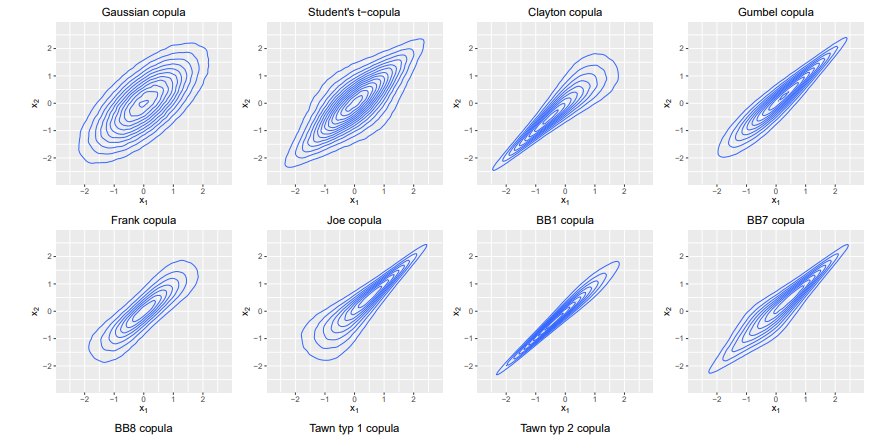
\includegraphics[scale=0.5]{taildep.png}
	\label{fig:fig1}
\end{figure}

\end{frame}

\begin{frame}
\frametitle{Methodology: Mixed Copula}

	\begin{enumerate}[(3)]
	\justifying
	
	\setbeamercovered{transparent}
	
	\pause
		
		\item Take the first derivative of the copula function to compute conditional
		probabilities and measure mispricing degrees $MI_{X\mid Y}$ and $MI_{Y\mid X}$ for each day.
		
		% in the trading period using the copula and estimated parameters.
		
		\vspace{0.3cm}
		
	\end{enumerate}

	\pause
	\begin{enumerate}[(4)]
	\justifying
		
		\item Build long and short positions of $Y$ and $X$ on the days that $M_{1,t}>\Delta_{1}$ and $M_{2,t}<\Delta_{2}$ if there is no positions in $X$ or $Y$. 
		
		\vspace{0.1cm}
		\begin{itemize}
			\item Conversely, build positions long/short of $X$ and $Y$ on the day that $M_{1,t}<\Delta_{2}$ and $M_{2,t}>\Delta_{1}$ if there is no positions in $X$ or $Y$.
		\end{itemize}
		
	\end{enumerate}

	\pause
		\begin{itemize}
	\item  All positions are closed if $M_{1,t}$ reaches $\Delta_{3}$ or $M_{2,t}$ reaches $\Delta_{4}$, where $\Delta_{1},\Delta_{2},\Delta_{3}$ and $\Delta_{4}$ are predetermined thresholds or are automatically closed out on the last day of the trading period if they do not reach the thresholds. 
	
	\vspace{0.3cm}
	\pause
	
	\item Here we use $\Delta_{1}=0.2, \Delta_{2}=-0.2$ and $\Delta_{3}=\Delta_{4}=0$.
	
	\end{itemize}
	
\end{frame}

	\begin{frame}
\frametitle{Illustration}

\begin{figure}[htbp]
	\centering
	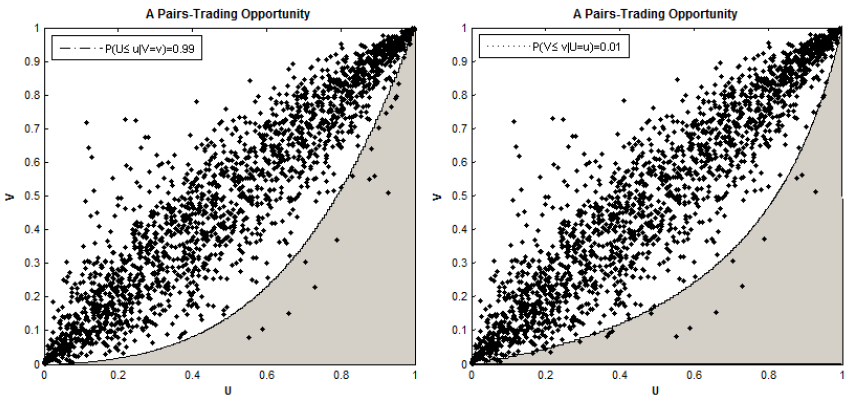
\includegraphics[scale=0.33]{trading_opt.png}
	\label{fig:trad_opt}
\end{figure}

\begin{figure}[htbp]
	\centering
	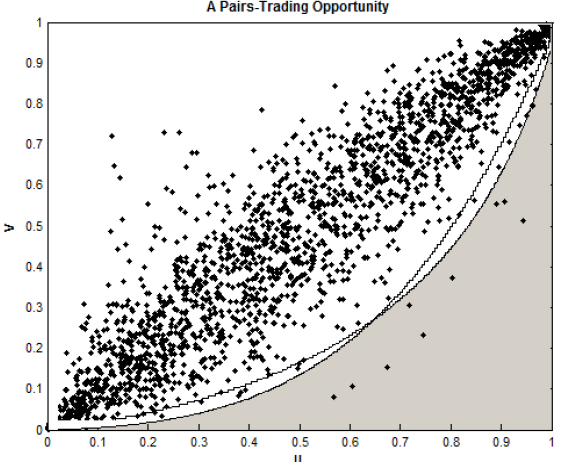
\includegraphics[scale=0.33]{trading_opt2.png}
	\label{fig:trad_opt2}
\end{figure}

\end{frame}



\section{Empirical Results}

\begin{frame}
	\frametitle{Risk-Return characteristics}
	
	\begin{figure}[!ht]
		\centering
		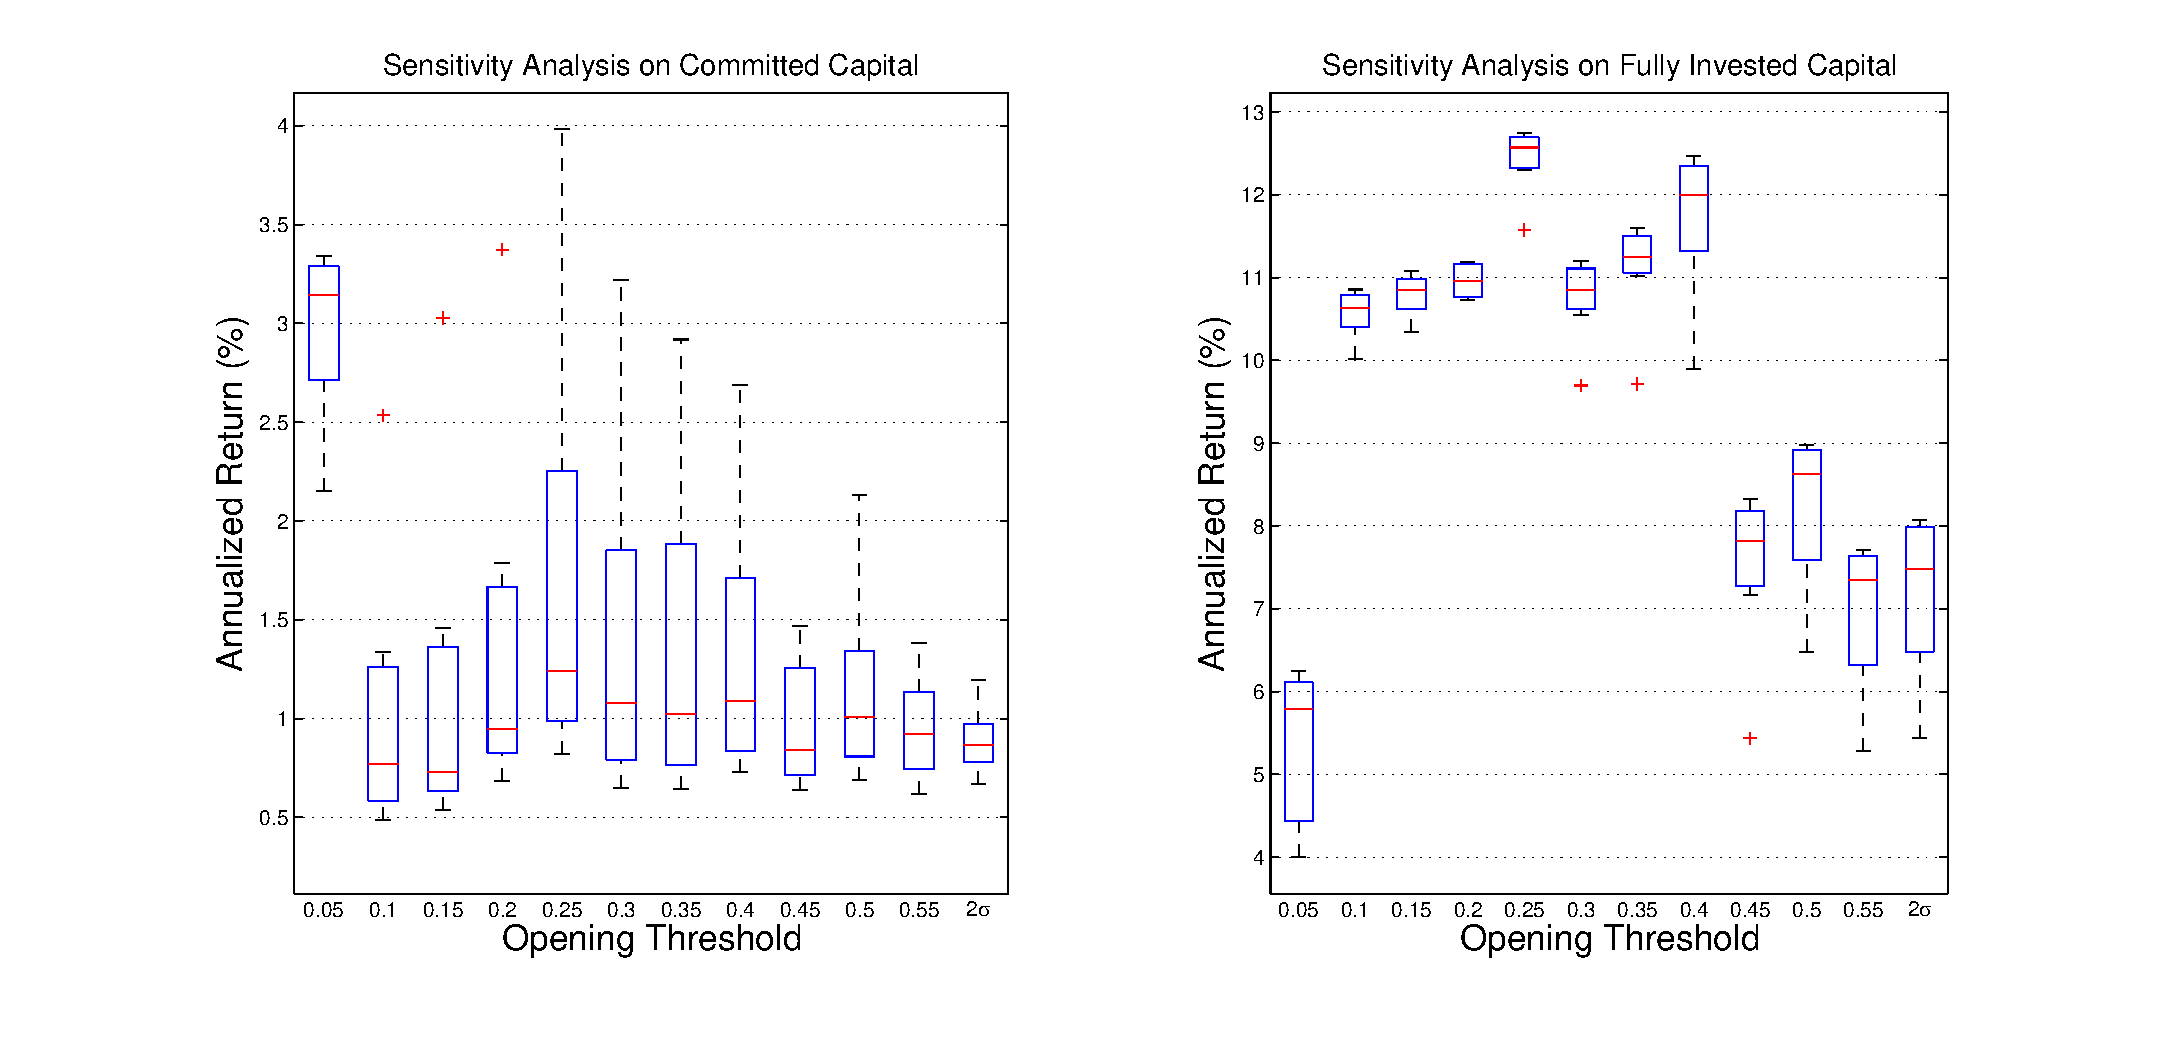
\includegraphics[width=12cm,height=5cm]{Figure1.eps}
		\captionsetup{justification=raggedright,
			singlelinecheck=false
		}
		\caption{\textbf{Annualized returns of pairs trading strategies after costs on committed and fully invested capital}}
		\caption*{\scriptsize These boxplots show annualized returns on committed (left) and fully invested (right) capital after transaction cost to different opening thresholds from July 1991 to December 2015 for Top 5 to Top 35 pairs.}
		\label{fig:fig1}
	\end{figure}

\end{frame}

\begin{frame}
	\frametitle{Risk-Return characteristics}
	
	\begin{figure}[!ht]
		\centering
		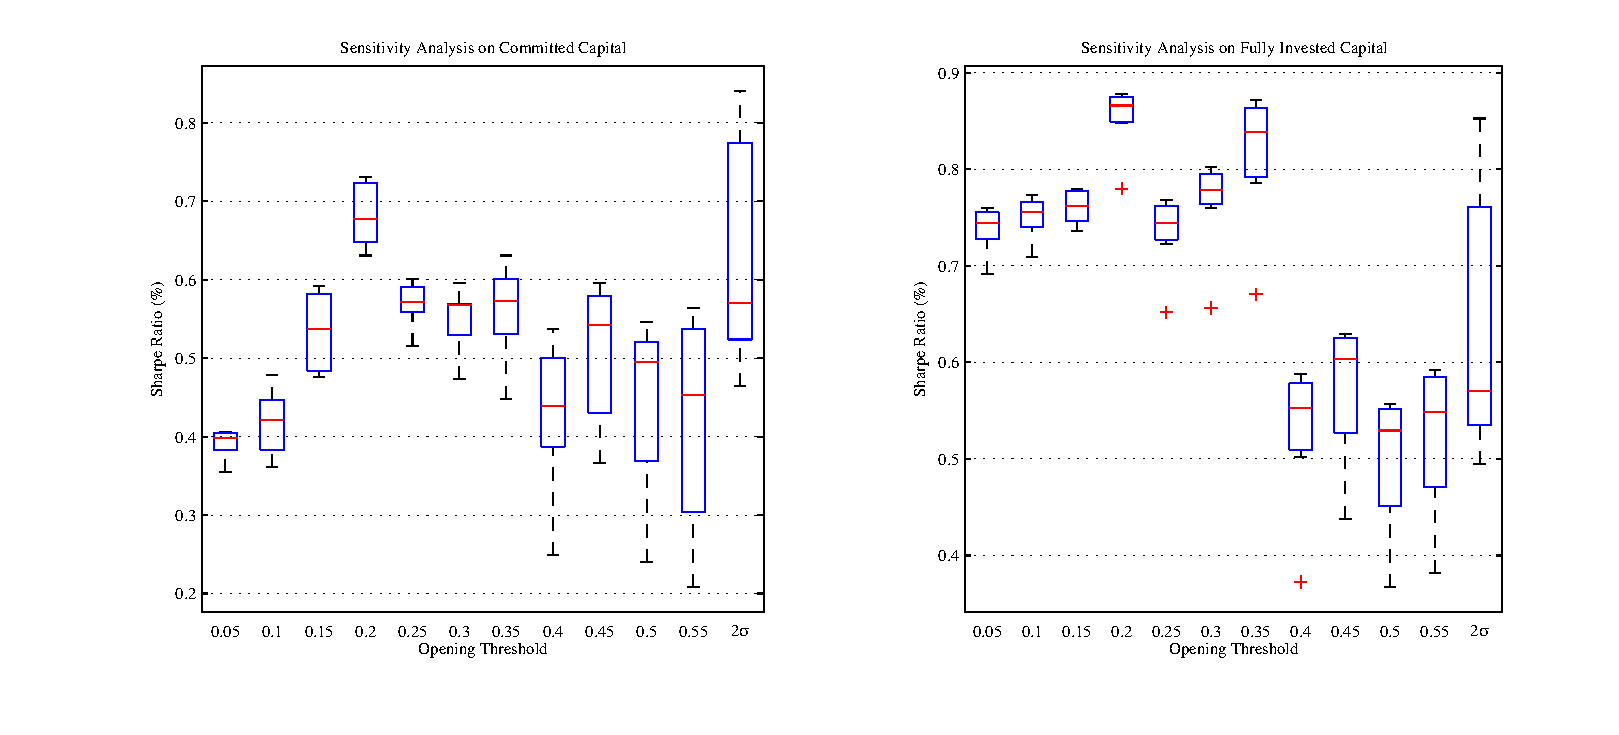
\includegraphics[width=12cm,height=5cm]{Figure2.eps}
		\captionsetup{justification=raggedright,
			singlelinecheck=false
		}
		\caption{\textbf {Sharpe ratio of pairs trading strategies after costs on committed and fully invested capital}}
%		\caption* {\scriptsize These boxplots show Sharpe ratios on committed (left) and fully invested (right) capital after transaction cost to different opening thresholds from July 1991 to December 2015 for Top 5 to Top 35 pairs. Pairs are formed based on the smallest sum of squared deviations.}
		\label{fig:fig2}
	\end{figure}
	
\end{frame}

\begin{frame}

\definecolor{corn}{rgb}{0.98, 0.93, 0.36}
\definecolor{celadon}{rgb}{0.67, 0.88, 0.69}
\frametitle{Trading Statistics}

\begin{threeparttable}[H]
	\centering \scriptsize
	\caption{Trading statistics.}
	\begin{tabularx}{\textwidth}{@{\extracolsep{\fill}}p{5cm}p{1cm}p{1cm}p{1cm}p{1cm}@{}}
		\toprule
		\multicolumn{1}{c}{Strategy} & Distance & Mixed Copula \\
		\midrule
		& \multicolumn{4}{c}{\textit{Panel A: Top 5}} \\
		& &  \\
		Average price deviation trigger for opening pairs & 0.0594 & 0.0665  \\
		Total number of pairs opened & \cellcolor{corn} 352   & \cellcolor{corn} 348   \\
		Average number of pairs traded per 6-month & 7.18 & 7.10    \\
		Average number of round-trip trades per pair & 1.44 & 1.42   \\
		~~Standard Deviation & 1.0128 & 1.33   \\
		Average time pairs are open in days & \cellcolor{corn} 50.70 & \cellcolor{corn} 37.70  \\
		~~Standard Deviation & 39.24 & 38.93    \\
		Median time pairs are open in days & \cellcolor{corn} 38.5  & \cellcolor{corn} 19          \\
		& &  \\
		& &  \\
		& \multicolumn{4}{c}{\textit{Panel B: Top20}} \\
		& & \\
		Average price deviation trigger for opening pairs & 0.0681 & 0.0821    \\
		Total number of pairs opened & \cellcolor{celadon} 1312  & \cellcolor{celadon} 749     \\
		Average number of pairs traded per 6-month & 26.78 & 15.29   \\
		Average number of round-trip trades per pair & 1.34 & 0.76  \\
		~Standard Deviation & 0.99 & 0.99    \\
		Average time pairs are open in days & 51.65 & 23.60   \\
		~Standard Deviation & 39.62 & 32.90    \\
		Median time pairs are open in days & 41    & 9           \\
		& & \\
		& \multicolumn{4}{c}{\textit{Panel C: Top 35}} \\
		& & \\
		Average price deviation trigger for opening pairs & 0.0729 & 0.0893   \\
		Total number of pairs opened & 2238  & 941   \\
		Average number of pairs traded per 6-month & 45.68 & 19.20 \\
		Average number of round-trip trades per pair & 1.30 & 0.55   \\
		~Standard Deviation & 1.02 & 0.84   \\
		Average time pairs are open in days & 52.72 &  19.35   \\
		~Standard Deviation & 40.48 & 30.56  \\
		Median time pairs are open in days & 42    & 6           \\
		\bottomrule
	\end{tabularx}%
	\begin{tablenotes}
		\item \textit{Note:} \scriptsize  Trading statistics for portfolio of top 5, 20 and 35 pairs between July 1991 and December 2015 (49 periods). Pairs are formed over a 12-month period according to a minimum-distance (sum of squared deviations) criterion and then traded over the subsequent 6-month period. Average price deviation trigger for opening a pair is calculated as the price difference divided by the average of the prices.
	\end{tablenotes}
	\label{tab:table105}%
\end{threeparttable}%

\end{frame}

\begin{frame}

\definecolor{corn}{rgb}{0.98, 0.93, 0.36}
\definecolor{celadon}{rgb}{0.67, 0.88, 0.69}
\frametitle{Trading Statistics}

\begin{threeparttable}[H]
\centering \scriptsize
\caption{Trading statistics.}
\begin{tabularx}{\textwidth}{@{\extracolsep{\fill}}p{5cm}p{1cm}p{1cm}p{1cm}p{1cm}@{}}
	\toprule
	\multicolumn{1}{c}{Strategy} & Distance & Mixed Copula \\
	\midrule
	& \multicolumn{4}{c}{\textit{Panel C: Top 35}} \\
	& & \\
	Average price deviation trigger for opening pairs & 0.0729 & 0.0893   \\
	Total number of pairs opened & \cellcolor{celadon} 2238  & \cellcolor{celadon} 941   \\
	Average number of pairs traded per six-month period & 45.68 & 19.20 \\
	Average number of round-trip trades per pair & 1.30 & 0.55   \\
	~Standard Deviation & 1.02 & 0.84   \\
	Average time pairs are open in days & 52.72 &  19.35   \\
	~Standard Deviation & 40.48 & 30.56  \\
	Median time pairs are open in days & 42    & 6           \\
	\bottomrule
\end{tabularx}%
\begin{tablenotes}
	\item \textit{Note:} \tiny  Trading statistics for portfolio of top 5, 20 and 35 pairs between July 1991 and December 2015 (49 periods). Pairs are formed over a 12-month period according to a minimum-distance (sum of squared deviations) criterion and then traded over the subsequent 6-month period. Average price deviation trigger for opening a pair is calculated as the price difference divided by the average of the prices.
\end{tablenotes}
\label{tab:table106}%
\end{threeparttable}%

\end{frame}

	\begin{frame}
		
		\definecolor{corn}{rgb}{0.98, 0.93, 0.36}
		\definecolor{celadon}{rgb}{0.67, 0.88, 0.69}
		
		\frametitle{Empirical Results}
			\begin{threeparttable}[H]
			\centering \tiny
			\caption{Excess returns on committed capital of pairs trading strategies on portfolios of Top 5, 20 and 35 pairs after costs. }
			\begin{tabularx}{\textwidth}{@{\extracolsep{\fill}}llllllll@{}}
				\toprule
				Strategy & Mean  & Sharpe & Sortino & t-stat & \% of negative   & MDD1 & MDD2 \\
				& Return (\% ) & ratio &  ratio     &  &  trades     &       &  \\
				\midrule
				\multicolumn{8}{c}{\textbf{Return on Committed Capital}} \\
				\multicolumn{8}{c}{\textit{Panel A - Top 5 pairs}} \\
				&       &       &       &       &       &       &  \\
				Distance & 2.60  & 0.31  & 0.58  & $1.86^{*}$  & 46.98 & 6.73    & 19.62 \\
				Mixed Copula & \cellcolor{corn} 3.98  & \cellcolor{corn} 0.63  & 1.08  & \cellcolor{corn} $3.49^{***}$  & \cellcolor{corn} 41.79 & \cellcolor{corn} 4.36  & \cellcolor{corn} 9.29 \\
				\multicolumn{1}{r}{} & \multicolumn{1}{r}{} & \multicolumn{1}{r}{} & \multicolumn{1}{r}{} & \multicolumn{1}{r}{} & \multicolumn{1}{r}{} & \multicolumn{1}{r}{} & \multicolumn{1}{r}{} \\
				\multicolumn{8}{c}{\textit{Panel B - Top 20 pairs}} \\
				&       &       &       &       &       &       &  \\
				Distance & \cellcolor{celadon} 3.14  & \cellcolor{celadon} 0.65  & 1.13  & $3.32^{***}$  & 48.02 & 3.88  & 9.69 \\
				Mixed Copula  & 1.24  & 0.64  & 1.04  & $3.52^{***}$  & 41.33 & \cellcolor{corn} 2.07  & \cellcolor{corn} 3.43  \\
				\multicolumn{1}{r}{} & \multicolumn{1}{r}{} & \multicolumn{1}{r}{} & \multicolumn{1}{r}{} & \multicolumn{1}{r}{} & \multicolumn{1}{r}{} & \multicolumn{1}{r}{} & \multicolumn{1}{r}{} \\
				\multicolumn{8}{c}{\textit{Panel C - Top 35 pairs}} \\
				&       &       &       &       &       &       &  \\
				Distance & \cellcolor{celadon} 3.12  & \cellcolor{celadon} 0.77  & 1.36  & $3.92^{***}$  & 47.97 & 2.70  & 7.52 \\
				Mixed Copula & 0.82  & 0.73  & 1.19  & $3.95^{***}$  & 41.31 & \cellcolor{corn} 1.18  & \cellcolor{corn} 1.98  \\
				\multicolumn{1}{r}{} & \multicolumn{1}{r}{} & \multicolumn{1}{r}{} & \multicolumn{1}{r}{} & \multicolumn{1}{r}{} & \multicolumn{1}{r}{} & \multicolumn{1}{r}{} & \multicolumn{1}{r}{} \\
				\midrule
				S\&P 500  & 4.36  & \cellcolor{Melon} 0.23  & 0.52  & $1.79^{*}$  & 47.45 & \cellcolor{Melon} 12.42  & \cellcolor{Melon} 46.74  \\
				\bottomrule
			\end{tabularx}%
			\begin{tablenotes}
				\item \textit{Note:} \scriptsize \tiny Summary statistics of the annualized excess returns, annualized Sharpe and Sortino ratios on portfolios of top 5, 20 and 35 pairs between July 1991 and December 2015 (6,173 observations). The t-statistics are computed using Newey-West standard errors with a six-lag correction. The columns labeled MDD1 and MDD2 compute the largest drawdown in terms of maximum percentage drop between two consecutive days and between two days within a period of maximum six months, respectively.
				\item \scriptsize $^{\ast\ast\ast}$, $^{\ast\ast}$, $^{\ast}$  significant at 1\%, 5\% and 10\% levels, respectively.
			\end{tablenotes}
			\label{tab:table101}%
		\end{threeparttable}%

	\end{frame}

\begin{frame}
	\definecolor{corn}{rgb}{0.98, 0.93, 0.36}
	\definecolor{celadon}{rgb}{0.67, 0.88, 0.69}
	\frametitle{Empirical Results}
	\begin{threeparttable}[H]
		\centering \tiny
		\caption{Excess returns on fully invested capital of pairs trading strategies on portfolios of Top 5, 20 and 35 pairs after costs. }
		\begin{tabularx}{\textwidth}{@{\extracolsep{\fill}}llllllll@{}}
			\toprule
			Strategy & Mean  & Sharpe & Sortino & t-stat & \% of negative   & MDD1 & MDD2 \\
			& Return (\% ) & ratio &  ratio     &  &  trades     &       &  \\
			\midrule
			\multicolumn{8}{c}{\textbf{Return on Fully Invested Capital}} \\
			\multicolumn{8}{c}{\textit{Panel A - Top 5 pairs}} \\
			&       &       &       &       &       &       &  \\
			Distance & 4.01  & 0.28  & 0.57  & $1.81^{*}$  & 46.98 & 8.70    & 38.36  \\
			Mixed Copula & 11.58  & 0.78  & 1.43  & $4.26^{***}$  & 41.79 & 9.00  & 25.68 \\
			\multicolumn{1}{r}{} & \multicolumn{1}{r}{} & \multicolumn{1}{r}{} & \multicolumn{1}{r}{} & \multicolumn{1}{r}{} & \multicolumn{1}{r}{} & \multicolumn{1}{r}{} & \multicolumn{1}{r}{} \\
			\multicolumn{8}{c}{\textit{Panel B - Top 20 pairs}} \\
			&       &       &       &       &       &       &  \\
			Distance & 6.07  & 0.66  & 1.19  & $3.55^{***}$  & 48.06 & 5.43  & 20.03 \\
			Mixed Copula  & 12.30  & 0.85  & 1.54  & $4.60^{***}$  & 41.31 & 9.00  & 25.68  \\
			\multicolumn{1}{r}{} & \multicolumn{1}{r}{} & \multicolumn{1}{r}{} & \multicolumn{1}{r}{} & \multicolumn{1}{r}{} & \multicolumn{1}{r}{} & \multicolumn{1}{r}{} & \multicolumn{1}{r}{} \\
			\multicolumn{8}{c}{\textit{Panel C - Top 35 pairs}} \\
			&       &       &       &       &       &       &  \\
			Distance & 5.76  & 0.76  & 1.38  & $4.05^{***}$  & 47.97 & 4.24  & 15.07 \\
			Mixed Copula & 12.73  & 0.88  & 1.59  & $4.73^{***}$  & 41.28 & 9.00  & 25.68  \\
			\multicolumn{1}{r}{} & \multicolumn{1}{r}{} & \multicolumn{1}{r}{} & \multicolumn{1}{r}{} & \multicolumn{1}{r}{} & \multicolumn{1}{r}{} & \multicolumn{1}{r}{} & \multicolumn{1}{r}{} \\
			\bottomrule
		\end{tabularx}%
		\begin{tablenotes}
%			\item \textit{Note:} \tiny Summary statistics of the annualized excess returns, annualized Sharpe and Sortino ratios on portfolios of top 5, 20 and 35 pairs between July 1991 and December 2015 (6,173 observations). Pairs are formed based on the smallest sum of squared deviations. The t-statistics are computed using Newey-West standard errors with a six-lag correction. The columns labeled MDD1 and MDD2 compute the largest drawdown in terms of maximum percentage drop between two consecutive days and between two days within a period of maximum six months, respectively.
			\item \scriptsize $^{\ast\ast\ast}$, $^{\ast\ast}$, $^{\ast}$  significant at 1\%, 5\% and 10\% levels, respectively.
		\end{tablenotes}
		\label{tab:table103}%
	\end{threeparttable}%

\end{frame}


\begin{frame}[label=frame5a]
\frametitle{Cumulative excess returns of pairs trading strategies after costs}

\begin{figure}[!ht]
	\centering
	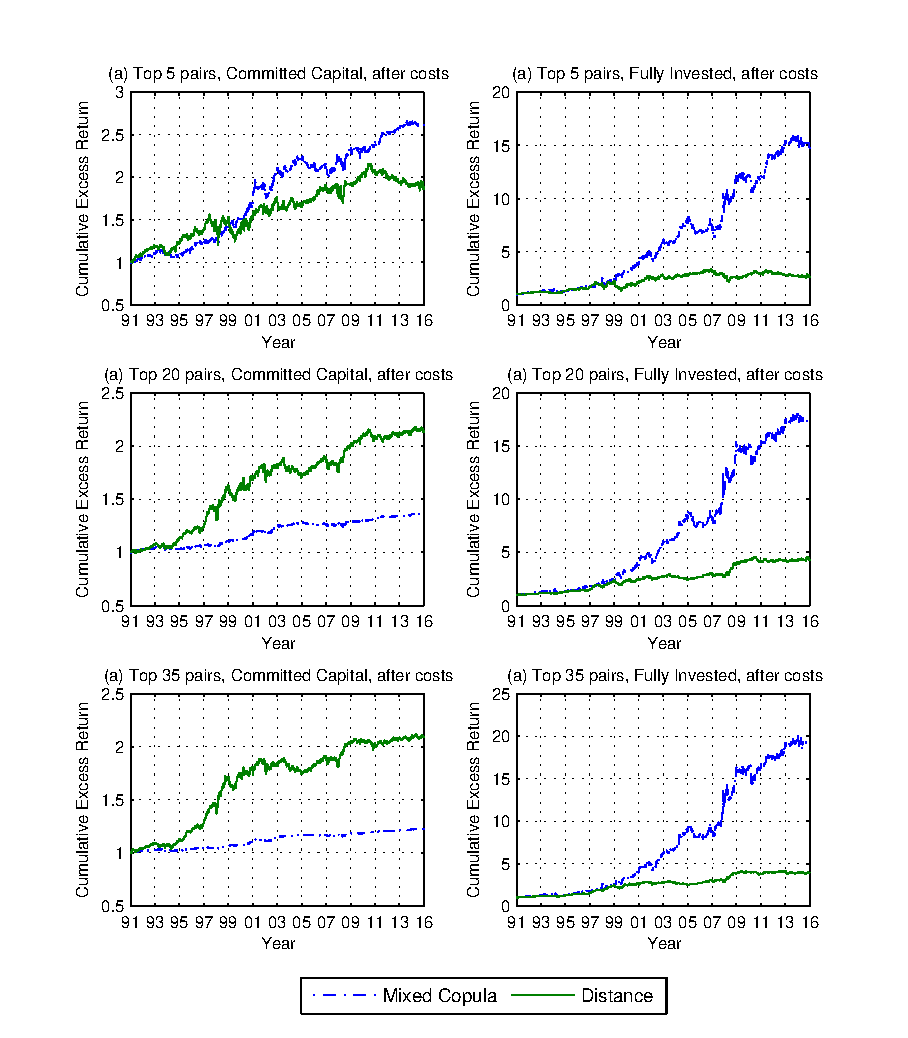
\includegraphics[scale=0.46]{Figure3.eps}
	\captionsetup{justification=raggedright,
		singlelinecheck=false
	}
%	\caption{\textbf{Cumulative excess returns of pairs trading strategies after costs}}
	\caption*{\tiny This figure shows how an investment of \$1 evolves from July 1991 to December 2015 for each of the strategies.}
	\label{fig:fig3}
\end{figure}

\end{frame}


\begin{frame}[label=frame5c]
\frametitle{Kernel density estimation of 5-year rolling window Sharpe ratio after costs}

\begin{figure}[!ht]
	\centering
	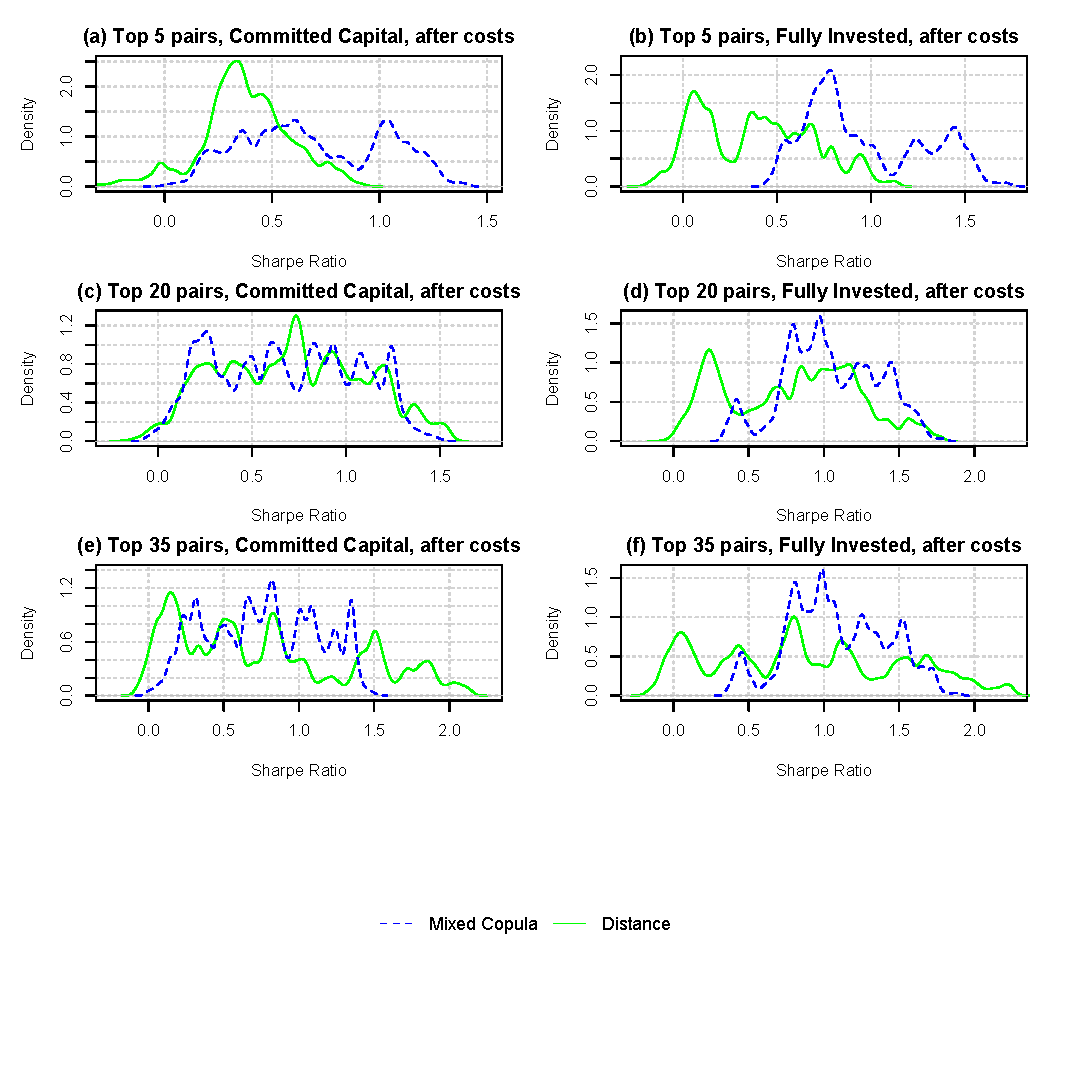
\includegraphics[scale=0.47]{Figure5.eps}
	\captionsetup{justification=raggedright,
		singlelinecheck=false
	}
%	\caption{\textbf{Kernel density estimation of 5-year rolling window Sharpe ratio after costs}}
	\caption*{\tiny  This figure shows how the 5-year rolling window Sharpe ratio densities evolve from July 1996 to December 2015 for each of the strategies with Sheather and Jones (1991)'s bandwidths.}
	\label{fig:fig5}
\end{figure}

\end{frame}


\section{Fama-French}

\begin{frame}

\setbeamercovered{transparent}

\definecolor{corn}{rgb}{0.98, 0.93, 0.36}
\definecolor{celadon}{rgb}{0.67, 0.88, 0.69}
\frametitle{Fama-French}

\begin{table}
	\centering \srcsize
	\caption{Monthly risk profile of Top 5 pairs: \textcolor{blue}{Fama and French} \textcolor{blue}{(2016)}'s five factors plus Momentum and Long-Term Reversal.}\label{tab:table103}%
	\begin{threeparttable}[!ht]
		\begin{tabularx}{\textwidth}{@{\extracolsep{\fill}} lllllllllll@{}}
			\toprule
			\multicolumn{1}{c}{Strategy} & \multicolumn{1}{c}{Intercept} &  \multicolumn{1}{c}{Rm-Rf} &  \multicolumn{1}{c}{SMB} &  \multicolumn{1}{c}{HML} &  \multicolumn{1}{c}{RMW} &  \multicolumn{1}{c}{CMA} & 
			\multicolumn{1}{c}{Mom} &  \multicolumn{1}{c}{LRev} &  \multicolumn{1}{c}{$R^{2}$} & \multicolumn{1}{c}{$R^{2}_{adj}$} \\
			\midrule
			\multicolumn{11}{c}{\textbf{Section 1: Return on Committed Capital}} \\
			\multicolumn{1}{c}{} & \multicolumn{1}{c}{} & \multicolumn{1}{c}{} & \multicolumn{1}{c}{} & \multicolumn{1}{c}{} & \multicolumn{1}{c}{} & \multicolumn{1}{c}{} & \multicolumn{1}{c}{} & \multicolumn{1}{c}{} & \multicolumn{1}{c}{} & \\
			\multicolumn{1}{c}{Distance} & 0.0025 & 0.0091 & -0.0032 & 0.0113 & 0.0003 & -0.0029 & -0.0107 & -0.0084 & 0.028 & 0.027 \\
			\multicolumn{1}{c}{} & $(1.89)^{*}$ & $(4.22)^{***}$ & (-0.71) & $(2.05)^{**}$ & (0.25) & (-0.18) & $(-4.80)^{***}$ & $(-1.96)^{**}$ & & \\
			\multicolumn{1}{c}{Mixed Copula} &  \cellcolor{corn} 0.0035 & \cellcolor{corn} 0.0052 & -0.0043 & 0.0039 & -0.0035 & 0.0027 & -0.0054 & -0.0057 & \cellcolor{corn} 0.015 &  \cellcolor{corn} 0.014 \\
			\multicolumn{1}{c} {}&  $(3.55)^{***}$ & $(3.68)^{***}$ & $(-1.83)^{*}$ & (1.20) & (-0.99) & (0.63) & $(-2.99)^{***}$ & (-1.57) &  & \\
			
			&       &       &       &       &       &       &       &       &       &       \\
			\midrule
			\multicolumn{11}{c}{\textbf{Section 2: Return on Fully Invested Capital}} \\
			&       &       &       &       &       &       &       &       &       &    \\
			\multicolumn{1}{c}{Distance} & 0.0040 & 0.0170 & -0.0031 & 0.0185 & 0.0049 & -0.0018 & -0.0161 & -0.0150 & 0.025 & 0.024 \\
			\multicolumn{1}{c}{} & $(1.75)^{*}$ & $(4.88)^{***}$ & (-0.45) & $(2.22)^{**}$ & (0.76) & (0.05) & $(-4.30)^{***}$ & $(-1.97)^{**}$ & & \\
			
			\multicolumn{1}{c}{Mixed Copula} & \cellcolor{corn} 0.0098 & \cellcolor{corn} 0.0148 & -0.0084 & 0.0152 & -0.0053 & 0.0087 & -0.0082 & -0.0222 & 0.018 & 0.017 \\
			\multicolumn{1}{c} {}&  $(4.17)^{***}$ & $(3.51)^{***}$ & -1.45 & 1.6355 & -0.60 & 0.75 & $(-2.19)^{**}$ & $(-2.08)^{**}$ & & \\
			\bottomrule
		\end{tabularx}
		\begin{tablenotes}
%			\item \tiny Note: This table shows results of regressing monthly portfolio return series onto \textcolor{blue}{Fama and French} \textcolor{blue}{(2016)}'s five factors factors plus momentum and long-term reversal over July 1991 and December 2015 (6173 observations). Section 1 shows the Return on Committed Capital and Section 2 on Fully Invested Capital after transaction costs. Pairs are formed based on the smallest sum of squared deviations. The t-statistics (shown in parentheses) are computed using Newey-West standard errors with six lags.
			\item \tiny $^{\ast\ast\ast}$, $^{\ast\ast}$, $^{\ast}$  significant at 1\%, 5\% and 10\% levels, respectively.
		\end{tablenotes}
	\end{threeparttable}%
\end{table}%

\pause

\begin{itemize}
	\item Alphas are significantly positive and higher than the raw excess returns by about 2-7 bps per month.
	
	\pause 
	\begin{itemize}
		\item Only a small part of the excess returns can be attributed to their exposures to the seven risk determinants.
	\end{itemize}
\end{itemize}

%We find that the, of the regressions, indicating that

\end{frame}

\section{Conclusions}

\begin{frame}[label=frame5b2]
\frametitle{Conclusions}

\setbeamercovered{transparent}

\begin{enumerate}
	%\setcounter{enumi}{1}
	\justifying
	
	
	\item By capturing linear/nonlinear associations and covering a wider range of possible dependencies structures, the mixed copula strategy outperforms the distance method when the number of trading signals is equiparable, especially after the subprime mortgage crisis.
	
	\pause
	\vspace{0.3cm}
	
	\item We show that the mixed copula pairs trading strategy generates large and significant (at 1\%) abnormal returns.
	
	\pause
		\begin{itemize}
			\item Only a small part of the pairs trading profits can be explained by market portfolio (beta), size (SMB), value (HML), investment (CMA), profitability (RMW), momentum (Mom) and reversal (LRev) based factors.
		\end{itemize}
	
	%\item The alphas of all strategies remain large and significant even after several asset pricing factors such as market portfolio (beta), size (SMB), value (HML), investment(CMA), profitability (RMW), momentum (Mom) and reversal (LRev) are taken into account.
	
	%We find that abnormal returns are most pronounced in emerging markets on the one hand and in markets with a large number of eligible pairs on the other hand
	
\end{enumerate}

\end{frame}


\begin{frame}
	\frametitle{Extensions}
	
\begin{itemize}
%	\item Varying Threshold
	
%	\vspace{0.3cm}
	
	\item Copula-based arbitrage for triplets to increase information dependency information and measure relative pricing more comprehensively.
	
	%Create similar 
	
		\begin{figure}[htbp]
		\centering
		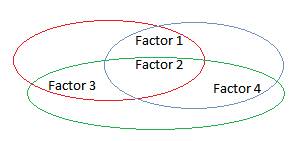
\includegraphics[scale=0.6]{fig4.png}
		\label{fig:fig4}
	\end{figure}

	\item Vine Copulas (Pair-Copula Constructions)
	
	\begin{itemize}
		\item Superior flexibility
	\end{itemize}
	
\end{itemize}
	
\end{frame}

\begin{frame}
\frametitle{Extensions}

	\begin{figure}[htbp]
	\centering
%	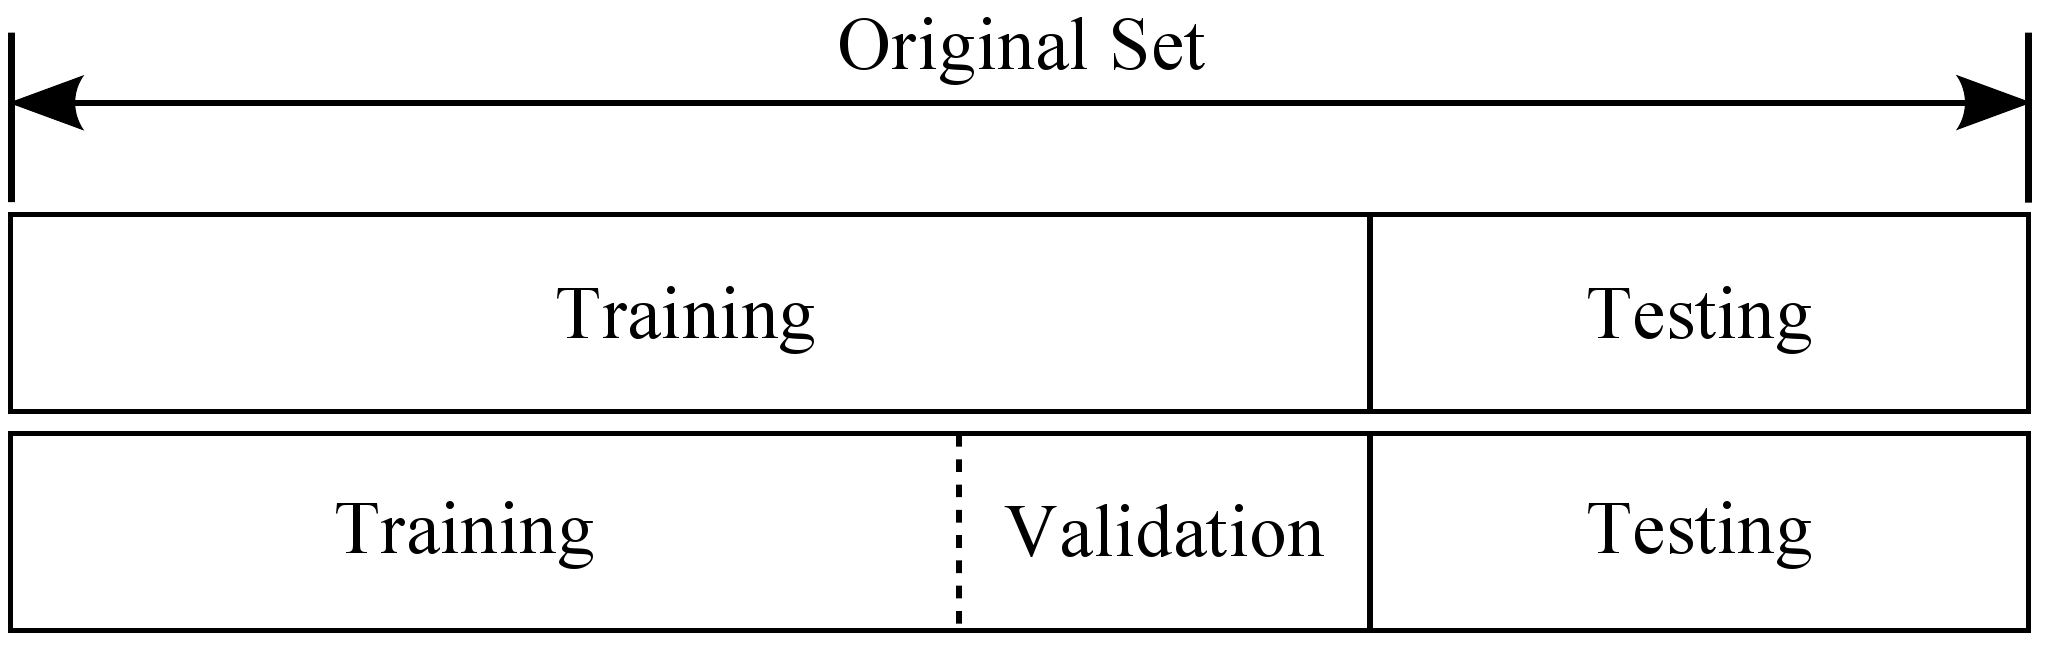
\includegraphics[scale=0.14]{fig3.png}

\includegraphics[scale=0.35]{man_machine2.png}
	\label{fig:fig3}
\end{figure}

\begin{itemize}
		\item Machine Learning and AI-based solutions (Man + Machine and NOT Man vs Machine) 
		%(e.g. learning automata)
	%\begin{itemize}
	%	\item Explore non-linear approaches
	%\end{itemize}
\vspace{0.3cm}
	\item News Sentiment
	\begin{itemize}
%		\item Contain relevant information about the economic activity
%		\item Can provide increased risk-adjusted returns
       % \item Sentiment-based long/short strategies
		\item Enhances a pairs-trading strategy using an abnormal news volume and sentiment overlay
		\item Effect of negative news is bigger than positive news and can lead to bigger sell-offs (asymmetry)
	\end{itemize}
	

	
\end{itemize}

\end{frame}

\begin{frame}

	\centering
	\Large{Thank you! Questions?}
	
\end{frame}

\appendix
\backupbegin

\begin{frame}
\definecolor{corn}{rgb}{0.98, 0.93, 0.36}

\frametitle{Subperiod Analysis}
\begin{threeparttable}[H]
	\centering \tiny
	\caption{Excess returns on committed capital on portfolios of Top 5 pairs after costs. }
	\begin{tabularx}{\textwidth}{@{\extracolsep{\fill}}llll@{}}
		\toprule
		Strategy & Mean  & Sharpe & Sortino \\
		& Return (\% ) & ratio &  ratio     \\
		\midrule
		\multicolumn{4}{c}{\textbf{Return on Committed Capital}} \\
		\multicolumn{4}{c}{\textit{Panel A: 1991-1995}} \\
		&       &       &       \\
		S\&P 500 & 7.17  & 0.72  & 1.30 \\
		Mixed Copula & 2.66  & 0.45  & 0.74 \\
		\multicolumn{1}{r}{} & \multicolumn{1}{r}{} & \multicolumn{1}{r}{} & \multicolumn{1}{r}{} \\
		\multicolumn{4}{c}{\textit{Panel B: 1996-2000}} \\
		&       &       &       \\
		S\&P 500 & 10.03  & 0.51  & 1.01 \\
		Mixed Copula & 6.90  & 1.05  & 1.77 \\
		\multicolumn{1}{r}{} & \multicolumn{1}{r}{} & \multicolumn{1}{r}{} & \multicolumn{1}{r}{} \\
		\multicolumn{4}{c}{\textit{Panel C: 2001-2005}} \\
		&       &       &       \\
		S\&P 500 & -2.28  & \cellcolor{Melon} -0.13  & -0.06 \\
		Mixed Copula & 6.84  & \cellcolor{corn} 0.83  & 1.44 \\
		\multicolumn{1}{r}{} & \multicolumn{1}{r}{} & \multicolumn{1}{r}{} & \multicolumn{1}{r}{} \\
		\multicolumn{4}{c}{\textit{Panel D: 2006:2010}} \\
		&       &       &       \\
		S\&P 500 & -1.71  & \cellcolor{Melon} -0.07  & 0.09 \\
		Mixed Copula & 1.56  & \cellcolor{corn} 0.24  & 0.46 \\
		\multicolumn{1}{r}{} & \multicolumn{1}{r}{} & \multicolumn{1}{r}{} & \multicolumn{1}{r}{} \\
		\multicolumn{4}{c}{\textit{Panel E: 2011:2015}} \\
		&       &       &       \\
		S\&P 500 & 9.91  & 0.61  & 1.09 \\
		Mixed Copula & 2.01  & 0.61  & 1.08 \\
		\multicolumn{1}{r}{} & \multicolumn{1}{r}{} & \multicolumn{1}{r}{} & \multicolumn{1}{r}{} \\
		\bottomrule
	\end{tabularx}%
	\begin{tablenotes}
		\item \scriptsize $^{\ast\ast\ast}$, $^{\ast\ast}$, $^{\ast}$  significant at 1\%, 5\% and 10\% levels, respectively.
	\end{tablenotes}
	\label{tab:table106}%
\end{threeparttable}%

\end{frame}

\begin{frame}

\frametitle{Subperiod Analysis}
\definecolor{corn}{rgb}{0.98, 0.93, 0.36}

\begin{threeparttable}[H]
	\centering \tiny
	\caption{Excess returns on fully invested capital on portfolios of Top 5 pairs after costs. }
	\begin{tabularx}{\textwidth}{@{\extracolsep{\fill}}llll@{}}
		\toprule
		Strategy & Mean  & Sharpe & Sortino \\
		& Return (\% ) & ratio &  ratio     \\
		\midrule
		\multicolumn{4}{c}{\textbf{Return on Fully Invested Capital}} \\
		\multicolumn{4}{c}{\textit{Panel A: 1991-1995}} \\
		&       &       &       \\
		S\&P 500 & 7.17  & 0.72  & 1.30 \\
		Mixed Copula & 7.69  & 0.56  & 1.02 \\
		\multicolumn{1}{r}{} & \multicolumn{1}{r}{} & \multicolumn{1}{r}{} & \multicolumn{1}{r}{} \\
		\multicolumn{4}{c}{\textit{Panel B: 1996-2000}} \\
		&       &       &       \\
		S\&P 500 & 10.03  & 0.51  & 1.01 \\
		Mixed Copula & 19.61  & 1.13  & 1.96 \\
		\multicolumn{1}{r}{} & \multicolumn{1}{r}{} & \multicolumn{1}{r}{} & \multicolumn{1}{r}{} \\
		\multicolumn{4}{c}{\textit{Panel C: 2001-2005}} \\
		&       &       &       \\
		S\&P 500 & -2.28  & \cellcolor{Melon} -0.13  & -0.06 \\
		Mixed Copula & 18.07  & \cellcolor{corn} 1.14  & 2.07 \\
		\multicolumn{1}{r}{} & \multicolumn{1}{r}{} & \multicolumn{1}{r}{} & \multicolumn{1}{r}{} \\
		\multicolumn{4}{c}{\textit{Panel D: 2006:2010}} \\
		&       &       &       \\
		S\&P 500 & -1.71  & \cellcolor{Melon} -0.07  & 0.09 \\
		Mixed Copula & 9.42  & \cellcolor{corn} 0.57  & 1.16 \\
		\multicolumn{1}{r}{} & \multicolumn{1}{r}{} & \multicolumn{1}{r}{} & \multicolumn{1}{r}{} \\
		\multicolumn{4}{c}{\textit{Panel E: 2011:2015}} \\
		&       &       &       \\
		S\&P 500 & 9.91  & 0.61  & 1.09 \\
		Mixed Copula & 3.62  & 0.37  & 0.69 \\
		\multicolumn{1}{r}{} & \multicolumn{1}{r}{} & \multicolumn{1}{r}{} & \multicolumn{1}{r}{} \\
		\bottomrule
	\end{tabularx}%
	\begin{tablenotes}
		\item \scriptsize $^{\ast\ast\ast}$, $^{\ast\ast}$, $^{\ast}$  significant at 1\%, 5\% and 10\% levels, respectively.
	\end{tablenotes}
	\label{tab:table107}%
\end{threeparttable}%

\end{frame}

\begin{frame}
\definecolor{corn}{rgb}{0.98, 0.93, 0.36}

\frametitle{Subperiod Analysis}
\begin{threeparttable}[H]
	\centering \tiny
	\caption{Excess returns on committed capital on portfolios of Top 20 pairs after costs. }
	\begin{tabularx}{\textwidth}{@{\extracolsep{\fill}}llll@{}}
		\toprule
		Strategy & Mean  & Sharpe & Sortino \\
		& Return (\% ) & ratio &  ratio     \\
		\midrule
		\multicolumn{4}{c}{\textbf{Return on Committed Capital}} \\
		\multicolumn{4}{c}{\textit{Panel A: 1991-1995}} \\
		&       &       &       \\
		S\&P 500 & 7.17  & 0.72  & 1.30 \\
		Mixed Copula & 0.93  & 0.46  & 0.70 \\
		\multicolumn{1}{r}{} & \multicolumn{1}{r}{} & \multicolumn{1}{r}{} & \multicolumn{1}{r}{} \\
		\multicolumn{4}{c}{\textit{Panel B: 1996-2000}} \\
		&       &       &       \\
		S\&P 500 & 10.03  & 0.51  & 1.01 \\
		Mixed Copula & 1.67  & 0.84  & 1.37 \\
		\multicolumn{1}{r}{} & \multicolumn{1}{r}{} & \multicolumn{1}{r}{} & \multicolumn{1}{r}{} \\
		\multicolumn{4}{c}{\textit{Panel C: 2001-2005}} \\
		&       &       &       \\
		S\&P 500 & -2.28  & \cellcolor{Melon} -0.13  & -0.06 \\
		Mixed Copula & 2.43  & \cellcolor{corn} 1.09  & 1.86 \\
		\multicolumn{1}{r}{} & \multicolumn{1}{r}{} & \multicolumn{1}{r}{} & \multicolumn{1}{r}{} \\
		\multicolumn{4}{c}{\textit{Panel D: 2006:2010}} \\
		&       &       &       \\
		S\&P 500 & -1.71  & \cellcolor{Melon} -0.07  & 0.09 \\
		Mixed Copula & 0.49  & \cellcolor{corn} 0.22  & 0.38 \\
		\multicolumn{1}{r}{} & \multicolumn{1}{r}{} & \multicolumn{1}{r}{} & \multicolumn{1}{r}{} \\
		\multicolumn{4}{c}{\textit{Panel E: 2011:2015}} \\
		&       &       &       \\
		S\&P 500 & 9.91  & 0.61  & 1.09 \\
		Mixed Copula & 0.70  & 0.77  & 1.30 \\
		\multicolumn{1}{r}{} & \multicolumn{1}{r}{} & \multicolumn{1}{r}{} & \multicolumn{1}{r}{} \\
		\bottomrule
	\end{tabularx}%
	\begin{tablenotes}
		\item \scriptsize $^{\ast\ast\ast}$, $^{\ast\ast}$, $^{\ast}$  significant at 1\%, 5\% and 10\% levels, respectively.
	\end{tablenotes}
	\label{tab:table108}%
\end{threeparttable}%

\end{frame}

\begin{frame}

\frametitle{Subperiod Analysis}
\definecolor{corn}{rgb}{0.98, 0.93, 0.36}

\begin{threeparttable}[H]
\centering \tiny
\caption{Excess returns on fully invested capital on portfolios of Top 20 pairs after costs. }
\begin{tabularx}{\textwidth}{@{\extracolsep{\fill}}llll@{}}
	\toprule
	Strategy & Mean  & Sharpe & Sortino \\
	& Return (\% ) & ratio &  ratio     \\
	\midrule
	\multicolumn{4}{c}{\textbf{Return on Fully Invested Capital}} \\
	\multicolumn{4}{c}{\textit{Panel A: 1991-1995}} \\
	&       &       &       \\
	S\&P 500 & 7.17  & 0.72  & 1.30 \\
	Mixed Copula & 8.18  & 0.63  & 1.10 \\
	\multicolumn{1}{r}{} & \multicolumn{1}{r}{} & \multicolumn{1}{r}{} & \multicolumn{1}{r}{} \\
	\multicolumn{4}{c}{\textit{Panel B: 1996-2000}} \\
	&       &       &       \\
	S\&P 500 & 10.03  & 0.51  & 1.01 \\
	Mixed Copula & 18.48  & 1.08  & 1.85 \\
	\multicolumn{1}{r}{} & \multicolumn{1}{r}{} & \multicolumn{1}{r}{} & \multicolumn{1}{r}{} \\
	\multicolumn{4}{c}{\textit{Panel C: 2001-2005}} \\
	&       &       &       \\
	S\&P 500 & -2.28  & \cellcolor{Melon} -0.13  & -0.06 \\
	Mixed Copula & 21.07  & \cellcolor{corn} 1.34  & 2.42 \\
	\multicolumn{1}{r}{} & \multicolumn{1}{r}{} & \multicolumn{1}{r}{} & \multicolumn{1}{r}{} \\
	\multicolumn{4}{c}{\textit{Panel D: 2006:2010}} \\
	&       &       &       \\
	S\&P 500 & -1.71  & \cellcolor{Melon} -0.07  & 0.09 \\
	Mixed Copula & 12.09  & \cellcolor{corn} 0.74  & 1.48 \\
	\multicolumn{1}{r}{} & \multicolumn{1}{r}{} & \multicolumn{1}{r}{} & \multicolumn{1}{r}{} \\
	\multicolumn{4}{c}{\textit{Panel E: 2011:2015}} \\
	&       &       &       \\
	S\&P 500 & 9.91  & 0.61  & 1.09 \\
	Mixed Copula & 2.33  & 0.25  & 0.49 \\
	\multicolumn{1}{r}{} & \multicolumn{1}{r}{} & \multicolumn{1}{r}{} & \multicolumn{1}{r}{} \\
	\bottomrule
\end{tabularx}%
\begin{tablenotes}
	\item \scriptsize $^{\ast\ast\ast}$, $^{\ast\ast}$, $^{\ast}$  significant at 1\%, 5\% and 10\% levels, respectively.
\end{tablenotes}
\label{tab:table109}%
\end{threeparttable}%

\end{frame}

\begin{frame}
\definecolor{corn}{rgb}{0.98, 0.93, 0.36}

\frametitle{Subperiod Analysis}
\begin{threeparttable}[H]
	\centering \tiny
	\caption{Excess returns on committed capital on portfolios of Top 35 pairs after costs. }
	\begin{tabularx}{\textwidth}{@{\extracolsep{\fill}}llll@{}}
		\toprule
		Strategy & Mean  & Sharpe & Sortino \\
		& Return (\% ) & ratio &  ratio     \\
		\midrule
		\multicolumn{4}{c}{\textbf{Return on Committed Capital}} \\
		\multicolumn{4}{c}{\textit{Panel A: 1991-1995}} \\
		&       &       &       \\
		S\&P 500 & 7.17  & 0.72  & 1.30 \\
		Mixed Copula & 0.70  & 0.60  & 0.93 \\
		\multicolumn{1}{r}{} & \multicolumn{1}{r}{} & \multicolumn{1}{r}{} & \multicolumn{1}{r}{} \\
		\multicolumn{4}{c}{\textit{Panel B: 1996-2000}} \\
		&       &       &       \\
		S\&P 500 & 10.03  & 0.51  & 1.01 \\
		Mixed Copula & 0.99  & 0.84  & 1.37 \\
		\multicolumn{1}{r}{} & \multicolumn{1}{r}{} & \multicolumn{1}{r}{} & \multicolumn{1}{r}{} \\
		\multicolumn{4}{c}{\textit{Panel C: 2001-2005}} \\
		&       &       &       \\
		S\&P 500 & -2.28  & \cellcolor{Melon} -0.13  & -0.06 \\
		Mixed Copula & 1.59  & \cellcolor{corn} 1.23  & 2.11 \\
		\multicolumn{1}{r}{} & \multicolumn{1}{r}{} & \multicolumn{1}{r}{} & \multicolumn{1}{r}{} \\
		\multicolumn{4}{c}{\textit{Panel D: 2006:2010}} \\
		&       &       &       \\
		S\&P 500 & -1.71  & \cellcolor{Melon} -0.07  & 0.09 \\
		Mixed Copula & 0.35  & \cellcolor{corn} 0.28  & 0.46 \\
		\multicolumn{1}{r}{} & \multicolumn{1}{r}{} & \multicolumn{1}{r}{} & \multicolumn{1}{r}{} \\
		\multicolumn{4}{c}{\textit{Panel E: 2011:2015}} \\
		&       &       &       \\
		S\&P 500 & 9.91  & 0.61  & 1.09 \\
		Mixed Copula & 0.50  & 0.86  & 1.56 \\
		\multicolumn{1}{r}{} & \multicolumn{1}{r}{} & \multicolumn{1}{r}{} & \multicolumn{1}{r}{} \\
		\bottomrule
	\end{tabularx}%
	\begin{tablenotes}
		\item \scriptsize $^{\ast\ast\ast}$, $^{\ast\ast}$, $^{\ast}$  significant at 1\%, 5\% and 10\% levels, respectively.
	\end{tablenotes}
	\label{tab:table110}%
\end{threeparttable}%

\end{frame}

\begin{frame}

\frametitle{Subperiod Analysis}
\definecolor{corn}{rgb}{0.98, 0.93, 0.36}

\begin{threeparttable}[H]
\centering \tiny
\caption{Excess returns on fully invested capital on portfolios of Top 35 pairs after costs. }
\begin{tabularx}{\textwidth}{@{\extracolsep{\fill}}llll@{}}
	\toprule
	Strategy & Mean  & Sharpe & Sortino \\
	& Return (\% ) & ratio &  ratio     \\
	\midrule
	\multicolumn{4}{c}{\textbf{Return on Fully Invested Capital}} \\
	\multicolumn{4}{c}{\textit{Panel A: 1991-1995}} \\
	&       &       &       \\
	S\&P 500 & 7.17  & 0.72  & 1.30 \\
	Mixed Copula & 8.50  & 0.65  & 1.14 \\
	\multicolumn{1}{r}{} & \multicolumn{1}{r}{} & \multicolumn{1}{r}{} & \multicolumn{1}{r}{} \\
	\multicolumn{4}{c}{\textit{Panel B: 1996-2000}} \\
	&       &       &       \\
	S\&P 500 & 10.03  & 0.51  & 1.01 \\
	Mixed Copula & 19.10  & 1.12  & 1.93 \\
	\multicolumn{1}{r}{} & \multicolumn{1}{r}{} & \multicolumn{1}{r}{} & \multicolumn{1}{r}{} \\
	\multicolumn{4}{c}{\textit{Panel C: 2001-2005}} \\
	&       &       &       \\
	S\&P 500 & -2.28  & \cellcolor{Melon} -0.13  & -0.06 \\
	Mixed Copula & 21.81  & \cellcolor{corn} 1.38  & 2.50 \\
	\multicolumn{1}{r}{} & \multicolumn{1}{r}{} & \multicolumn{1}{r}{} & \multicolumn{1}{r}{} \\
	\multicolumn{4}{c}{\textit{Panel D: 2006:2010}} \\
	&       &       &       \\
	S\&P 500 & -1.71  & \cellcolor{Melon} -0.07  & 0.09 \\
	Mixed Copula & 12.39  & \cellcolor{corn} 0.76  & 1.51 \\
	\multicolumn{1}{r}{} & \multicolumn{1}{r}{} & \multicolumn{1}{r}{} & \multicolumn{1}{r}{} \\
	\multicolumn{4}{c}{\textit{Panel E: 2011:2015}} \\
	&       &       &       \\
	S\&P 500 & 9.91  & 0.61  & 1.09 \\
	Mixed Copula & 2.56  & 0.27  & 0.53 \\
	\multicolumn{1}{r}{} & \multicolumn{1}{r}{} & \multicolumn{1}{r}{} & \multicolumn{1}{r}{} \\
	\bottomrule
\end{tabularx}%
\begin{tablenotes}
	\item \scriptsize $^{\ast\ast\ast}$, $^{\ast\ast}$, $^{\ast}$  significant at 1\%, 5\% and 10\% levels, respectively.
\end{tablenotes}
\label{tab:table111}%
\end{threeparttable}%

\end{frame}

\backupend

\end{document}







